\PassOptionsToPackage{unicode=true}{hyperref} % options for packages loaded elsewhere
\PassOptionsToPackage{hyphens}{url}
%
\documentclass[ignorenonframetext,]{beamer}
\usepackage{pgfpages}
\setbeamertemplate{caption}[numbered]
\setbeamertemplate{caption label separator}{: }
\setbeamercolor{caption name}{fg=normal text.fg}
\beamertemplatenavigationsymbolsempty
\usepackage{lmodern}
\usepackage{amssymb,amsmath}
\usepackage{ifxetex,ifluatex}
\usepackage{fixltx2e} % provides \textsubscript
\ifnum 0\ifxetex 1\fi\ifluatex 1\fi=0 % if pdftex
  \usepackage[T1]{fontenc}
  \usepackage[utf8]{inputenc}
  \usepackage{textcomp} % provides euro and other symbols
\else % if luatex or xelatex
  \usepackage{unicode-math}
  \defaultfontfeatures{Ligatures=TeX,Scale=MatchLowercase}
\fi
\usetheme[]{CambridgeUS}
\usecolortheme{beaver}
\usefonttheme{structurebold}
% use upquote if available, for straight quotes in verbatim environments
\IfFileExists{upquote.sty}{\usepackage{upquote}}{}
% use microtype if available
\IfFileExists{microtype.sty}{%
\usepackage[]{microtype}
\UseMicrotypeSet[protrusion]{basicmath} % disable protrusion for tt fonts
}{}
\IfFileExists{parskip.sty}{%
\usepackage{parskip}
}{% else
\setlength{\parindent}{0pt}
\setlength{\parskip}{6pt plus 2pt minus 1pt}
}
\usepackage{hyperref}
\hypersetup{
            pdftitle={osm main api},
            pdfauthor={Jan-Philipp Kolb},
            pdfborder={0 0 0},
            breaklinks=true}
\urlstyle{same}  % don't use monospace font for urls
\newif\ifbibliography
\usepackage{color}
\usepackage{fancyvrb}
\newcommand{\VerbBar}{|}
\newcommand{\VERB}{\Verb[commandchars=\\\{\}]}
\DefineVerbatimEnvironment{Highlighting}{Verbatim}{commandchars=\\\{\}}
% Add ',fontsize=\small' for more characters per line
\usepackage{framed}
\definecolor{shadecolor}{RGB}{248,248,248}
\newenvironment{Shaded}{\begin{snugshade}}{\end{snugshade}}
\newcommand{\AlertTok}[1]{\textcolor[rgb]{0.94,0.16,0.16}{#1}}
\newcommand{\AnnotationTok}[1]{\textcolor[rgb]{0.56,0.35,0.01}{\textbf{\textit{#1}}}}
\newcommand{\AttributeTok}[1]{\textcolor[rgb]{0.77,0.63,0.00}{#1}}
\newcommand{\BaseNTok}[1]{\textcolor[rgb]{0.00,0.00,0.81}{#1}}
\newcommand{\BuiltInTok}[1]{#1}
\newcommand{\CharTok}[1]{\textcolor[rgb]{0.31,0.60,0.02}{#1}}
\newcommand{\CommentTok}[1]{\textcolor[rgb]{0.56,0.35,0.01}{\textit{#1}}}
\newcommand{\CommentVarTok}[1]{\textcolor[rgb]{0.56,0.35,0.01}{\textbf{\textit{#1}}}}
\newcommand{\ConstantTok}[1]{\textcolor[rgb]{0.00,0.00,0.00}{#1}}
\newcommand{\ControlFlowTok}[1]{\textcolor[rgb]{0.13,0.29,0.53}{\textbf{#1}}}
\newcommand{\DataTypeTok}[1]{\textcolor[rgb]{0.13,0.29,0.53}{#1}}
\newcommand{\DecValTok}[1]{\textcolor[rgb]{0.00,0.00,0.81}{#1}}
\newcommand{\DocumentationTok}[1]{\textcolor[rgb]{0.56,0.35,0.01}{\textbf{\textit{#1}}}}
\newcommand{\ErrorTok}[1]{\textcolor[rgb]{0.64,0.00,0.00}{\textbf{#1}}}
\newcommand{\ExtensionTok}[1]{#1}
\newcommand{\FloatTok}[1]{\textcolor[rgb]{0.00,0.00,0.81}{#1}}
\newcommand{\FunctionTok}[1]{\textcolor[rgb]{0.00,0.00,0.00}{#1}}
\newcommand{\ImportTok}[1]{#1}
\newcommand{\InformationTok}[1]{\textcolor[rgb]{0.56,0.35,0.01}{\textbf{\textit{#1}}}}
\newcommand{\KeywordTok}[1]{\textcolor[rgb]{0.13,0.29,0.53}{\textbf{#1}}}
\newcommand{\NormalTok}[1]{#1}
\newcommand{\OperatorTok}[1]{\textcolor[rgb]{0.81,0.36,0.00}{\textbf{#1}}}
\newcommand{\OtherTok}[1]{\textcolor[rgb]{0.56,0.35,0.01}{#1}}
\newcommand{\PreprocessorTok}[1]{\textcolor[rgb]{0.56,0.35,0.01}{\textit{#1}}}
\newcommand{\RegionMarkerTok}[1]{#1}
\newcommand{\SpecialCharTok}[1]{\textcolor[rgb]{0.00,0.00,0.00}{#1}}
\newcommand{\SpecialStringTok}[1]{\textcolor[rgb]{0.31,0.60,0.02}{#1}}
\newcommand{\StringTok}[1]{\textcolor[rgb]{0.31,0.60,0.02}{#1}}
\newcommand{\VariableTok}[1]{\textcolor[rgb]{0.00,0.00,0.00}{#1}}
\newcommand{\VerbatimStringTok}[1]{\textcolor[rgb]{0.31,0.60,0.02}{#1}}
\newcommand{\WarningTok}[1]{\textcolor[rgb]{0.56,0.35,0.01}{\textbf{\textit{#1}}}}
\usepackage{longtable,booktabs}
\usepackage{caption}
% These lines are needed to make table captions work with longtable:
\makeatletter
\def\fnum@table{\tablename~\thetable}
\makeatother
\usepackage{graphicx,grffile}
\makeatletter
\def\maxwidth{\ifdim\Gin@nat@width>\linewidth\linewidth\else\Gin@nat@width\fi}
\def\maxheight{\ifdim\Gin@nat@height>\textheight\textheight\else\Gin@nat@height\fi}
\makeatother
% Scale images if necessary, so that they will not overflow the page
% margins by default, and it is still possible to overwrite the defaults
% using explicit options in \includegraphics[width, height, ...]{}
\setkeys{Gin}{width=\maxwidth,height=\maxheight,keepaspectratio}
% Prevent slide breaks in the middle of a paragraph:
\widowpenalties 1 10000
\raggedbottom
\setbeamertemplate{part page}{
\centering
\begin{beamercolorbox}[sep=16pt,center]{part title}
  \usebeamerfont{part title}\insertpart\par
\end{beamercolorbox}
}
\setbeamertemplate{section page}{
\centering
\begin{beamercolorbox}[sep=12pt,center]{part title}
  \usebeamerfont{section title}\insertsection\par
\end{beamercolorbox}
}
\setbeamertemplate{subsection page}{
\centering
\begin{beamercolorbox}[sep=8pt,center]{part title}
  \usebeamerfont{subsection title}\insertsubsection\par
\end{beamercolorbox}
}
\AtBeginPart{
  \frame{\partpage}
}
\AtBeginSection{
  \ifbibliography
  \else
    \frame{\sectionpage}
  \fi
}
\AtBeginSubsection{
  \frame{\subsectionpage}
}
\setlength{\emergencystretch}{3em}  % prevent overfull lines
\providecommand{\tightlist}{%
  \setlength{\itemsep}{0pt}\setlength{\parskip}{0pt}}
\setcounter{secnumdepth}{0}

% set default figure placement to htbp
\makeatletter
\def\fps@figure{htbp}
\makeatother


\title{osm main api}
\author{Jan-Philipp Kolb}
\date{23 Oktober 2018}

\begin{document}
\frame{\titlepage}

\begin{frame}{\href{http://www.openstreetmap.org/export}{OSM Ausschnitte
herunterladen}}
\protect\hypertarget{osm-ausschnitte-herunterladen}{}

\textless{}www.openstreetmap.org/export\textgreater{}

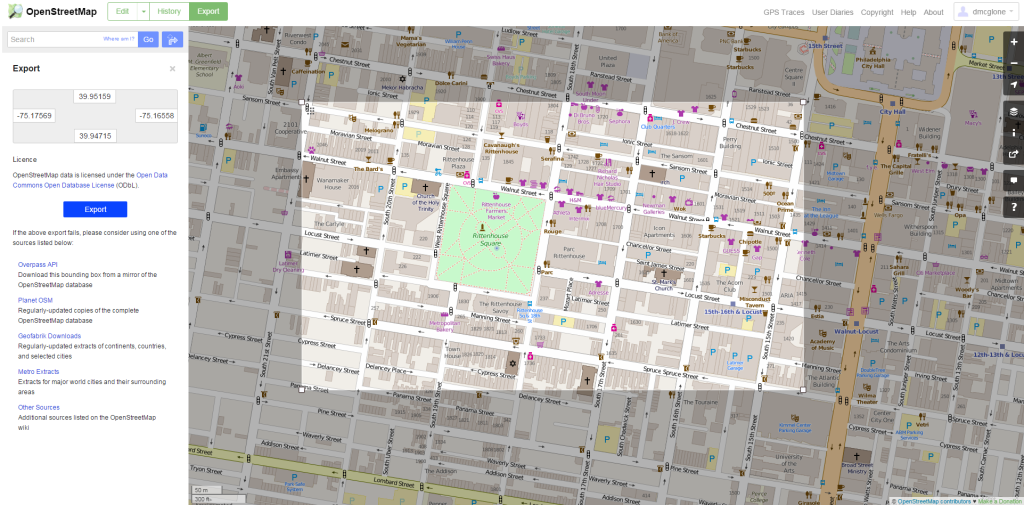
\includegraphics{figure/openstreetmap_export-1024x505.png}

\end{frame}

\begin{frame}[fragile]{Das R-Paket \texttt{XML} - Gaston Sanchez}
\protect\hypertarget{das-r-paket-xml---gaston-sanchez}{}

\begin{Shaded}
\begin{Highlighting}[]
\KeywordTok{library}\NormalTok{(}\StringTok{"XML"}\NormalTok{)}
\end{Highlighting}
\end{Shaded}

\begin{block}{Gaston Sanchez - Dataflow}

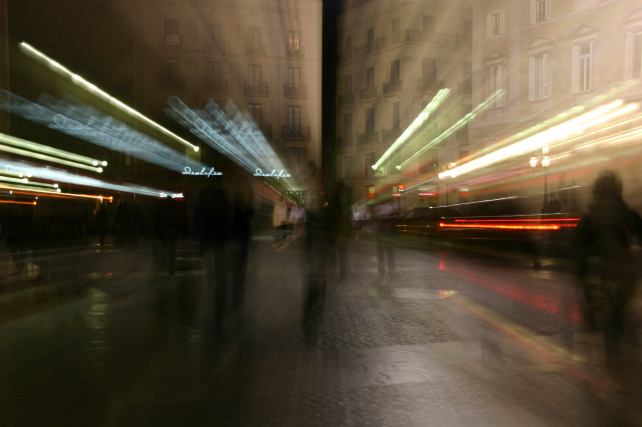
\includegraphics{figure/GastonSanchez2.png}

Seine Arbeit sieht man \href{http://gastonsanchez.com/}{\textbf{hier}}.

\end{block}

\end{frame}

\begin{frame}{\href{https://github.com/gastonstat/tutorial-R-web-data/blob/master/04-parsing-xml/04-parsing-xml.pdf}{Das
Arbeiten mit XML Daten}}
\protect\hypertarget{das-arbeiten-mit-xml-daten}{}

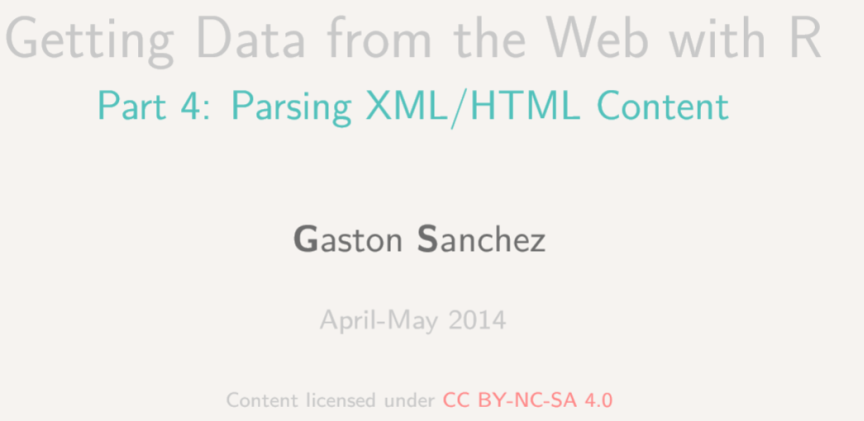
\includegraphics{figure/GastonSanchez3.PNG}

\end{frame}

\begin{frame}{Funktionen im XML Paket}
\protect\hypertarget{funktionen-im-xml-paket}{}

\begin{longtable}[]{@{}ll@{}}
\toprule
Function & Description\tabularnewline
\midrule
\endhead
xmlName() & name of the node\tabularnewline
xmlSize() & number of subnodes\tabularnewline
xmlAttrs() & named character vector of all attributes\tabularnewline
xmlGetAttr() & value of a single attribute\tabularnewline
xmlValue() & contents of a leaf node\tabularnewline
xmlParent() & name of parent node\tabularnewline
xmlAncestors() & name of ancestor nodes\tabularnewline
getSibling() & siblings to the right or to the left\tabularnewline
xmlNamespace() & the namespace (if there's one)\tabularnewline
\bottomrule
\end{longtable}

\end{frame}

\begin{frame}{\href{http://www.openstreetmap.org/export}{Einzelne
Objekte finden}}
\protect\hypertarget{einzelne-objekte-finden}{}

\textless{}www.openstreetmap.org/export\textgreater{}

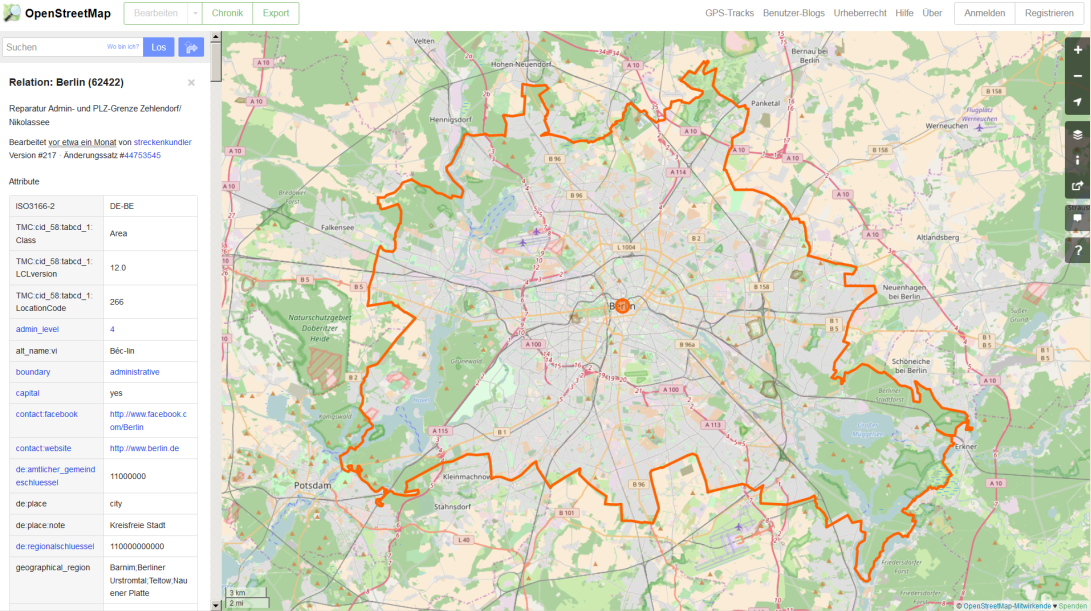
\includegraphics{figure/admgrBer.PNG}

\end{frame}

\begin{frame}[fragile]{Beispiel: administrative Grenzen Berlin}
\protect\hypertarget{beispiel-administrative-grenzen-berlin}{}

\href{http://wiki.openstreetmap.org/wiki/DE:Grenze\#Bundesl.C3.A4ndergrenze_-_admin_level.3D4}{Administrative
Grenzen für Deutschland}

\begin{Shaded}
\begin{Highlighting}[]
\NormalTok{url <-}\StringTok{ "https://api.openstreetmap.org/api/0.6/relation/62422"}
\end{Highlighting}
\end{Shaded}

\begin{Shaded}
\begin{Highlighting}[]
\NormalTok{BE <-}\StringTok{ }\KeywordTok{xmlParse}\NormalTok{(url)}
\end{Highlighting}
\end{Shaded}

\begin{Shaded}
\begin{Highlighting}[]
\NormalTok{BE <-}\StringTok{ }\KeywordTok{xmlParse}\NormalTok{(}\StringTok{"../data/62422.xml"}\NormalTok{)}
\end{Highlighting}
\end{Shaded}

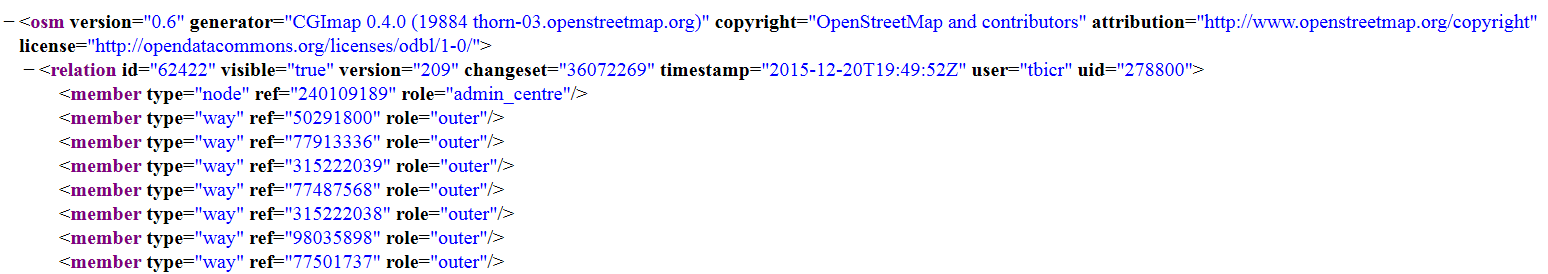
\includegraphics{figure/ExampleAdmBE.PNG}

\end{frame}

\begin{frame}[fragile]{Das XML analysieren}
\protect\hypertarget{das-xml-analysieren}{}

\begin{itemize}
\tightlist
\item
  \href{http://www.informit.com/articles/article.aspx?p=2215520}{Tobi
  Bosede - Working with XML Data in R}
\end{itemize}

\begin{Shaded}
\begin{Highlighting}[]
\NormalTok{xmltop =}\StringTok{ }\KeywordTok{xmlRoot}\NormalTok{(BE)}
\KeywordTok{class}\NormalTok{(xmltop)}
\end{Highlighting}
\end{Shaded}

\begin{verbatim}
## [1] "XMLInternalElementNode" "XMLInternalNode"       
## [3] "XMLAbstractNode"
\end{verbatim}

\begin{Shaded}
\begin{Highlighting}[]
\KeywordTok{xmlSize}\NormalTok{(xmltop)}
\end{Highlighting}
\end{Shaded}

\begin{verbatim}
## [1] 1
\end{verbatim}

\begin{Shaded}
\begin{Highlighting}[]
\KeywordTok{xmlSize}\NormalTok{(xmltop[[}\DecValTok{1}\NormalTok{]])}
\end{Highlighting}
\end{Shaded}

\begin{verbatim}
## [1] 337
\end{verbatim}

\end{frame}

\begin{frame}[fragile]{Nutzung von Xpath}
\protect\hypertarget{nutzung-von-xpath}{}

\begin{quote}
\href{https://de.wikipedia.org/wiki/XPath}{Xpath}, the XML Path
Language, is a query language for selecting nodes from an XML document.
\end{quote}

\begin{Shaded}
\begin{Highlighting}[]
\KeywordTok{xpathApply}\NormalTok{(BE,}\StringTok{"//tag[@k = 'population']"}\NormalTok{)}
\end{Highlighting}
\end{Shaded}

\begin{verbatim}
## [[1]]
## <tag k="population" v="3440441"/> 
## 
## attr(,"class")
## [1] "XMLNodeSet"
\end{verbatim}

\end{frame}

\begin{frame}[fragile]{Quelle für die Bevölkerungsgröße}
\protect\hypertarget{quelle-fur-die-bevolkerungsgroe}{}

\begin{Shaded}
\begin{Highlighting}[]
\KeywordTok{xpathApply}\NormalTok{(BE,}\StringTok{"//tag[@k = 'source:population']"}\NormalTok{)}
\end{Highlighting}
\end{Shaded}

\begin{verbatim}
## [[1]]
## <tag k="source:population" v="http://www.statistik-berlin-brandenburg.de/Publikationen/Stat_Berichte/2010/SB_A1-1_A2-4_q01-10_BE.pdf 2010-10-01"/> 
## 
## attr(,"class")
## [1] "XMLNodeSet"
\end{verbatim}

-\href{https://www.statistik-berlin-brandenburg.de/datenbank/inhalt-datenbank.asp}{\textbf{Statistik
Berlin Brandenburg}}

\end{frame}

\begin{frame}[fragile]{Etwas überraschend:}
\protect\hypertarget{etwas-uberraschend}{}

\begin{Shaded}
\begin{Highlighting}[]
\KeywordTok{xpathApply}\NormalTok{(BE,}\StringTok{"//tag[@k = 'name:ta']"}\NormalTok{)}
\end{Highlighting}
\end{Shaded}

\begin{verbatim}
## [[1]]
## <tag k="name:ta" v="<U+0BAA><U+0BC6><U+0BB0><U+0BCD><U+0BB2><U+0BBF><U+0BA9><U+0BCD>"/> 
## 
## attr(,"class")
## [1] "XMLNodeSet"
\end{verbatim}

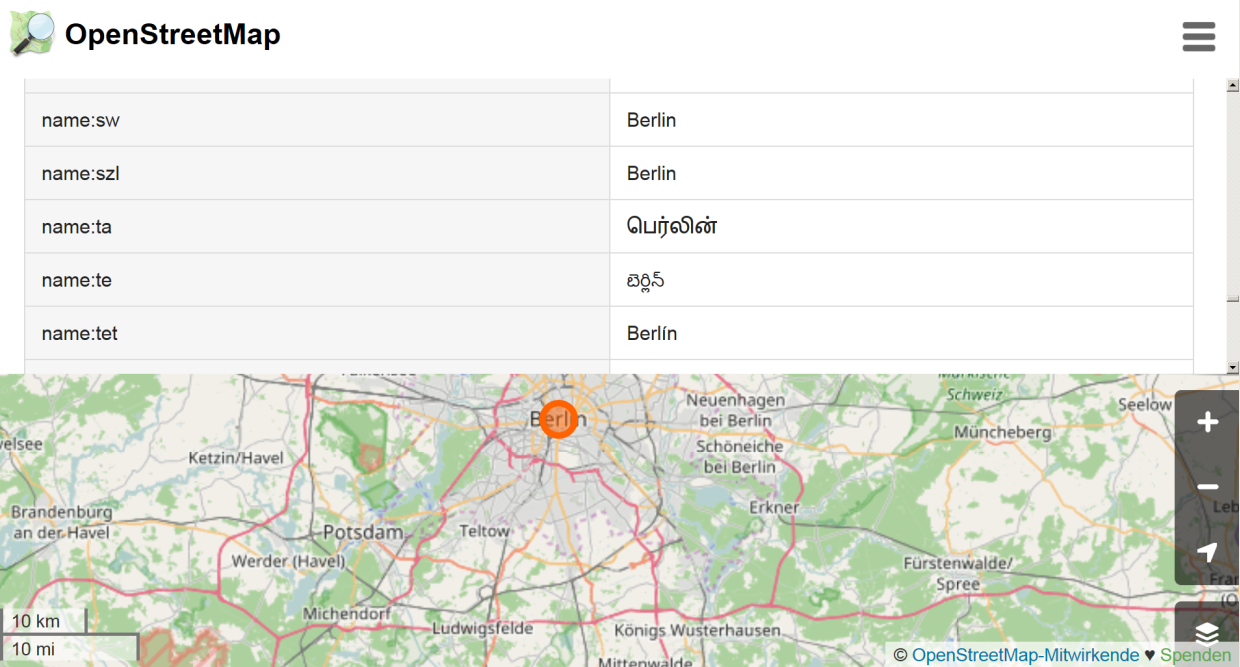
\includegraphics{figure/OSMBerta.png}

\end{frame}

\begin{frame}[fragile]{Geographische Region}
\protect\hypertarget{geographische-region}{}

\begin{Shaded}
\begin{Highlighting}[]
\NormalTok{region <-}\StringTok{ }\KeywordTok{xpathApply}\NormalTok{(BE,}
  \StringTok{"//tag[@k = 'geographical_region']"}\NormalTok{)}
\CommentTok{# regular expressions}
\NormalTok{region[[}\DecValTok{1}\NormalTok{]]}
\end{Highlighting}
\end{Shaded}

\begin{verbatim}
## <tag k="geographical_region" v="Barnim;Berliner Urstromtal;Teltow;Nauener Platte"/>
\end{verbatim}

\begin{verbatim}
<tag k="geographical_region" 
  v="Barnim;Berliner Urstromtal;
  Teltow;Nauener Platte"/>
\end{verbatim}

\end{frame}

\begin{frame}{Landkreis}
\protect\hypertarget{landkreis}{}

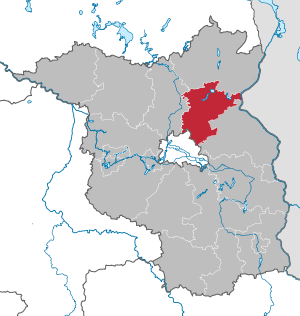
\includegraphics{figure/Barnim.png}

\end{frame}

\begin{frame}[fragile]{Weiteres Beispiel}
\protect\hypertarget{weiteres-beispiel}{}

\begin{Shaded}
\begin{Highlighting}[]
\NormalTok{url2<-}\StringTok{"http://api.openstreetmap.org/api/0.6/node/25113879"}
\NormalTok{obj2<-}\KeywordTok{xmlParse}\NormalTok{(url2)}
\NormalTok{obj_amenity<-}\KeywordTok{xpathApply}\NormalTok{(obj2,}\StringTok{"//tag[@k = 'amenity']"}\NormalTok{)[[}\DecValTok{1}\NormalTok{]]}
\NormalTok{obj_amenity}
\end{Highlighting}
\end{Shaded}

\begin{verbatim}
## <tag k="amenity" v="university"/>
\end{verbatim}

\end{frame}

\begin{frame}[fragile]{Wikipedia Artikel}
\protect\hypertarget{wikipedia-artikel}{}

\begin{Shaded}
\begin{Highlighting}[]
\KeywordTok{xpathApply}\NormalTok{(obj2,}\StringTok{"//tag[@k = 'wikipedia']"}\NormalTok{)[[}\DecValTok{1}\NormalTok{]]}
\end{Highlighting}
\end{Shaded}

\begin{verbatim}
## <tag k="wikipedia" v="de:Universität Mannheim"/>
\end{verbatim}

\begin{Shaded}
\begin{Highlighting}[]
\KeywordTok{xpathApply}\NormalTok{(obj2,}\StringTok{"//tag[@k = 'wheelchair']"}\NormalTok{)[[}\DecValTok{1}\NormalTok{]]}
\end{Highlighting}
\end{Shaded}

\begin{Shaded}
\begin{Highlighting}[]
\KeywordTok{xpathApply}\NormalTok{(obj2,}\StringTok{"//tag[@k = 'name']"}\NormalTok{)[[}\DecValTok{1}\NormalTok{]]}
\end{Highlighting}
\end{Shaded}

\end{frame}

\begin{frame}[fragile]{Das C und das A}
\protect\hypertarget{das-c-und-das-a}{}

\begin{Shaded}
\begin{Highlighting}[]
\NormalTok{url3<-}\StringTok{"http://api.openstreetmap.org/api/0.6/node/303550876"}
\NormalTok{obj3 <-}\StringTok{ }\KeywordTok{xmlParse}\NormalTok{(url3)}
\KeywordTok{xpathApply}\NormalTok{(obj3,}\StringTok{"//tag[@k = 'opening_hours']"}\NormalTok{)[[}\DecValTok{1}\NormalTok{]]}
\end{Highlighting}
\end{Shaded}

\begin{verbatim}
## <tag k="opening_hours" v="Mo-Sa 09:00-20:00; Su,PH off"/>
\end{verbatim}

\end{frame}

\begin{frame}[fragile]{Hin und weg}
\protect\hypertarget{hin-und-weg}{}

\begin{Shaded}
\begin{Highlighting}[]
\NormalTok{url4<-}\StringTok{"http://api.openstreetmap.org/api/0.6/node/25439439"}
\NormalTok{obj4 <-}\StringTok{ }\KeywordTok{xmlParse}\NormalTok{(url4)}
\KeywordTok{xpathApply}\NormalTok{(obj4,}\StringTok{"//tag[@k = 'railway:station_category']"}\NormalTok{)[[}\DecValTok{1}\NormalTok{]]}
\end{Highlighting}
\end{Shaded}

\begin{verbatim}
## <tag k="railway:station_category" v="2"/>
\end{verbatim}

\begin{itemize}
\tightlist
\item
  \href{https://de.wikipedia.org/wiki/Bahnhofskategorie}{\textbf{Wikipedia
  Artikel Bahnhofskategorien}}
\end{itemize}

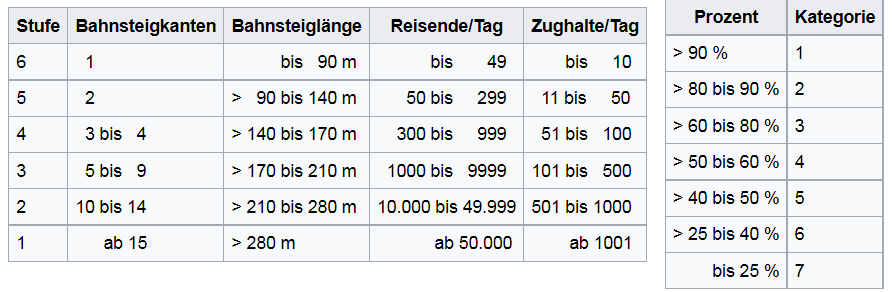
\includegraphics{figure/Bahnhofskategorien.PNG}

\end{frame}

\begin{frame}[fragile]{Exkurs: Bahnhofskategorien}
\protect\hypertarget{exkurs-bahnhofskategorien}{}

\begin{itemize}
\tightlist
\item
  \href{https://cran.r-project.org/web/packages/rvest/index.html}{\textbf{rvest:
  Easily Harvest (Scrape) Web Pages}}
\end{itemize}

\begin{Shaded}
\begin{Highlighting}[]
\KeywordTok{library}\NormalTok{(rvest)}
\end{Highlighting}
\end{Shaded}

\begin{verbatim}
## Loading required package: xml2
\end{verbatim}

\begin{verbatim}
## 
## Attaching package: 'rvest'
\end{verbatim}

\begin{verbatim}
## The following object is masked from 'package:XML':
## 
##     xml
\end{verbatim}

\begin{Shaded}
\begin{Highlighting}[]
\NormalTok{bhfkat<-}\KeywordTok{read_html}\NormalTok{(}
  \StringTok{"https://de.wikipedia.org/wiki/Bahnhofskategorie"}\NormalTok{)}
\NormalTok{df_html_bhfkat<-}\KeywordTok{html_table}\NormalTok{(}
  \KeywordTok{html_nodes}\NormalTok{(bhfkat, }\StringTok{"table"}\NormalTok{)[[}\DecValTok{2}\NormalTok{]],}\DataTypeTok{fill =} \OtherTok{TRUE}\NormalTok{)}
\end{Highlighting}
\end{Shaded}

\end{frame}

\begin{frame}{Bahnhofskategorien Übersicht}
\protect\hypertarget{bahnhofskategorien-ubersicht}{}

\begin{longtable}[]{@{}lllllll@{}}
\toprule
Stufe & Bahnsteigkanten & Bahnsteiglänge{[}Anm 1{]} & Reisende/Tag &
Zughalte/Tag & Service{[}Anm 2{]} & Stufenfreiheit{[}Anm
3{]}\tabularnewline
\midrule
\endhead
(0) & --- & --- & --- & --- & Nein & Nein\tabularnewline
1 & 01 & \textgreater{} 000 bis 090 m & 00.000 bis 00.049 & 000 bis 0010
& Ja & Ja\tabularnewline
2 & 02 & \textgreater{} 090 bis 140 m & 00.050 bis 00.299 & 011 bis 0050
& --- & ---\tabularnewline
3 & 03 bis 04 & \textgreater{} 140 bis 170 m & 00.300 bis 0.0999 & 051
bis 0100 & --- & ---\tabularnewline
4 & 05 bis 09 & \textgreater{} 170 bis 210 m & 01.000 bis 09.999 & 101
bis 0500 & --- & ---\tabularnewline
5 & 10 bis 14 & \textgreater{} 210 bis 280 m & 10.000 bis 49.999 & 501
bis 1000 & --- & ---\tabularnewline
6 & 00i ab 15 & \textgreater{} 280 m bis 000 & 000000 ab 50.000 & 000i
ab 1001 & --- & ---\tabularnewline
Gewichtung & 20~\% & 20~\% & 20~\% & 20~\% & 15~\% & 5~\%\tabularnewline
\bottomrule
\end{longtable}

\end{frame}

\begin{frame}[fragile]{Nur fliegen ist schöner}
\protect\hypertarget{nur-fliegen-ist-schoner}{}

\begin{Shaded}
\begin{Highlighting}[]
\NormalTok{url5<-}\StringTok{"http://api.openstreetmap.org/api/0.6/way/162149882"}
\NormalTok{obj5<-}\KeywordTok{xmlParse}\NormalTok{(url5)}
\KeywordTok{xpathApply}\NormalTok{(obj5,}\StringTok{"//tag[@k = 'name']"}\NormalTok{)[[}\DecValTok{1}\NormalTok{]]}
\end{Highlighting}
\end{Shaded}

\begin{verbatim}
## <tag k="name" v="City-Airport Mannheim"/>
\end{verbatim}

\begin{Shaded}
\begin{Highlighting}[]
\KeywordTok{xpathApply}\NormalTok{(obj5,}\StringTok{"//tag[@k = 'website']"}\NormalTok{)[[}\DecValTok{1}\NormalTok{]]}
\end{Highlighting}
\end{Shaded}

\begin{verbatim}
## <tag k="website" v="http://www.flugplatz-mannheim.de/"/>
\end{verbatim}

\begin{Shaded}
\begin{Highlighting}[]
\KeywordTok{xpathApply}\NormalTok{(obj5,}\StringTok{"//tag[@k = 'iata']"}\NormalTok{)[[}\DecValTok{1}\NormalTok{]]}
\end{Highlighting}
\end{Shaded}

\begin{verbatim}
## <tag k="iata" v="MHG"/>
\end{verbatim}

\end{frame}

\begin{frame}{Mehr Beispiele, wie man mit XML Daten umgeht:}
\protect\hypertarget{mehr-beispiele-wie-man-mit-xml-daten-umgeht}{}

\begin{itemize}
\item
  Deborah Nolan -
  \href{http://www.stat.berkeley.edu/~statcur/Workshop2/Presentations/XML.pdf}{\textbf{Extracting
  data from XML}}
\item
  Duncan Temple Lang -
  \href{http://www.omegahat.net/RSXML/shortIntro.pdf}{\textbf{A Short
  Introduction to the XML package for R}}
\end{itemize}

\begin{block}{Noch mehr Informationen}

\begin{itemize}
\item
  \href{http://www.di.fc.ul.pt/~jpn/r/web/index.html\#parsing-xml}{\textbf{Web
  Daten manipulieren}}
\item
  \href{http://www.w3schools.com/xml/xquery_intro.asp}{\textbf{Tutorial
  zu xquery}}
\item
  \href{http://giventhedata.blogspot.de/2012/06/r-and-web-for-beginners-part-ii-xml-in.html}{\textbf{R
  und das Web (für Anfänger), Teil II: XML und R}}
\item
  Gaston Sanchez -
  \href{http://gastonsanchez.com/Handling_and_Processing_Strings_in_R.pdf}{\textbf{String
  Manipulation}}
\item
  \href{https://www.e-education.psu.edu/geog585/node/738}{\textbf{Nutzung,
  Vor- und Nachteile OSM}}
\item
  \href{http://wiki.openstreetmap.org/wiki/Research}{\textbf{Forschungsprojekte
  im Zusammenhang mit OpenStreetMap}}
\end{itemize}

\end{block}

\end{frame}

\begin{frame}[fragile]{Referenzen}
\protect\hypertarget{referenzen}{}

\begin{Shaded}
\begin{Highlighting}[]
\KeywordTok{citation}\NormalTok{(}\StringTok{"XML"}\NormalTok{)}
\end{Highlighting}
\end{Shaded}

\begin{verbatim}
## 
## To cite package 'XML' in publications use:
## 
##   Duncan Temple Lang and the CRAN Team (2018). XML: Tools for
##   Parsing and Generating XML Within R and S-Plus. R package
##   version 3.98-1.11. https://CRAN.R-project.org/package=XML
## 
## A BibTeX entry for LaTeX users is
## 
##   @Manual{,
##     title = {XML: Tools for Parsing and Generating XML Within R and S-Plus},
##     author = {Duncan Temple Lang and the CRAN Team},
##     year = {2018},
##     note = {R package version 3.98-1.11},
##     url = {https://CRAN.R-project.org/package=XML},
##   }
## 
## ATTENTION: This citation information has been auto-generated from
## the package DESCRIPTION file and may need manual editing, see
## 'help("citation")'.
\end{verbatim}

\end{frame}

\begin{frame}[fragile]{Das neuere Paket}
\protect\hypertarget{das-neuere-paket}{}

\begin{Shaded}
\begin{Highlighting}[]
\KeywordTok{citation}\NormalTok{(}\StringTok{"xml2"}\NormalTok{)}
\end{Highlighting}
\end{Shaded}

\begin{verbatim}
## 
## To cite package 'xml2' in publications use:
## 
##   Hadley Wickham, James Hester and Jeroen Ooms (2018). xml2: Parse
##   XML. R package version 1.2.0.
##   https://CRAN.R-project.org/package=xml2
## 
## A BibTeX entry for LaTeX users is
## 
##   @Manual{,
##     title = {xml2: Parse XML},
##     author = {Hadley Wickham and James Hester and Jeroen Ooms},
##     year = {2018},
##     note = {R package version 1.2.0},
##     url = {https://CRAN.R-project.org/package=xml2},
##   }
\end{verbatim}

\end{frame}

\end{document}
